\chapter{Wat is een blockchain?}
\label{ch:wat-is-een-blockchain}

% Tip: Begin elk hoofdstuk met een paragraaf inleiding die beschrijft hoe
% dit hoofdstuk past binnen het geheel van de bachelorproef. Geef in het
% bijzonder aan wat de link is met het vorige en volgende hoofdstuk.

Dit hoofdstuk is het resultaat van een literatuurstudie, toegespitst op de eerste deelvraag van het onderzoek:

\begin{center}
	\textit{\textbf{``Wat is een blockchain?''}}
\end{center}

Vertrekkende vanuit het \textit{double-spendingprobleem}, wordt geïllustreerd dat het delen van een grootboek \textit{of ledger} onvermijdelijk voor vertrouwenskwesties zorgt. Dit issue werd voor geruime tijd enkel vanuit een gecentraliseerde systeem benaderd. Met het verlangen naar de eerste \textit{cryptocurrencies} ontstond de nood aan een gedecentraliseerde benadering. Een blockchain vormde de oplossing voor de problemen die daarbij kwamen opdagen.

Volgende secties werden opgebouwd met als doel een inzicht te geven in de structuur van een blockchain en hoe die structuur tot stand kwam. Daarom wordt vertrokken vanuit een veralgemeende probleemstelling. Door deze \textit{case} stelsel aan te vullen met enkele basisprincipes komen we uiteinlijk tot een oplossing onder de vorm van een blockchain. Deze basisprincipes weerspiegelen de implementatie van de eerste blockchain, zoals bedacht door Nakamoto. Op die manier toont dit hoofdstuk hoe een blockchain aan zijn eigenschappen komt. Wie deze eigenschappen in het achterhoofd houdt zal met een gefundeerd begrip de volgende deelvragen kunnen aanvatten.

% Pas na deze inleidende paragraaf komt de eerste sectiehoofding.


\section{Gedeelde ledgers}
\label{sec:probeleemstelling}
In de whitepaper ``Bitcoin: A Peer-to-Peer Electronic Cash System'' werkte Satoshi Nakamoto het voorstel uit van wat men vandaag een blockchain noemt. Met een vernuftige keten van datablokken loste Nakamoto het zogenaamde \textit{double-spendingprobleem} op. Het \textit{incentive} was om Bitcoin, de eerste gedecentraliseerde cryptomunt, uit te brengen. Voor dit onderzoek is het echter zinvol om de context zo min mogelijk vast te hangen aan \textit{cryptocurrencies}. Daarom zullen we het begrip ``transacties'' ook opentrekken naar andere toepassingsgebieden. Een veralgemeende probleemstelling rond zogenaamde \textit{ledgers} zal het vertrekpunt vormen van een meer technische uiteenzetting.


\subsection{Double-spending}
\label{sub:double-spending}

Double-spending is een probleem binnen de context van \textit{cryptocurrencies}. Het doet zich voor wanneer een partij eenzelfde digitale token voor meerdere transacties gebruikt, hoewel dit maar voor een het geval zou mogen zijn. Digitale munten kunnen namelijk (net zoals fysiek geld) gedupliceerd of vervalst worden. In tegenstelling tot tastbaar geld, bestaan digitale munten echter uitsluitend uit binaire data. Dat maakt de strijd tegen vervalsing extra uitdagend. Een kenteken van authenticiteit toevoegen, is op het eerste zicht niet mogelijk. Data kan namelijk heel gemakkelijk gerepliceerd worden. Een simpele aanduiding, analoog aan de zilverstrook op een bankbiljet, is bij een cryptomunt dus compleet zinloos. Het zou met een eenvoudige copy-paste kunnen vervalst worden. Om cryptomunten op de markt te brengen, waren dus andere oplossingen nodig.


\subsection{Transacties}
\label{sub:transacties}

In de oorspronkelijke toepassing van blockchains stond een transactie voor de bitcoin-overdracht van een partij naar een andere~\autocite{Pierro2017}. Er zijn echter veel meer transacties denkbaar dan enkel eenvoudige gelduitwisselingen.
In het boek ``Blockchain: Blueprint for a New Economy'' wordt blockchain-technologie opgedeeld in drie fases. De bijhorende toepassingsgebieden bepalen de transacties die denkbaar zijn om op te nemen in een blockchain~\autocite{Swan2015}.

\textbf{Blockchain 1.0} is het label voor blockchain-technologie, zoals die bestond in zijn oorspronkelijke context: cryptocurrencies. Een transactie staat in die context voor
\begin{itemize}
	\item het spenderen van een cryptomunt.
\end{itemize}
\textbf{Blockchain 2.0} staat voor een uitbreiding van de technologie, die voornamelijk beperkt blijft tot de financiële sector. Banken, betalingen en de \textit{supply chain} geeft aanleiding tot transacties zoals
\begin{itemize}
	\item afsluiten van \textit{smart contracts}
	\item uitwisselen van aandelen;
	\item uitwisselen van hypotheken;
	\item afsluiten van een abonnement;
	\item afsluiten van een verzekering;
	\item het versturen van een digitale factuur;
	\item ...
\end{itemize}
\textbf{Blockchain 3.0} wordt beschreven als de toepassing van blockchain in sectoren zoals gezondheidszorg, wetenschap, cultuur en de overheid. De uitwisseling die dan plaatsvindt gaat niet zozeer over financiële zaken, maar over informatie die ontstaat bij (s40854-019-0147-z.pdf)
\begin{itemize}
	\item de waarnemingen van een metaaldetector bij voedingsproductie;
	\item het toedienen van een inenting;
	\item het indienen van een subsidieaanvraag bij de overheid;
	\item ...
\end{itemize}

Ook al deze zaken horen uiteraard onvervalsbaar te zijn. Door het begrip transactie ruimer te bekijken, kan double-spending vertaald worden naar veralgemeende probleemstelling. Dit is zinvol, aangezien de \textit{use cases} voor dit onderzoek niet te vinden zijn in Blockchain 1.0, maar starten bij Blockchain 2.0.


\subsection{Probleemstelling}
\label{sub:casus}

In de gegeven context kunnen drie partijen onderlinge transacties uitvoeren. Er ontstaat nood aan een gedeeld grootboek of \textit{ledger} om al deze transacties in op te nemen. In deze ledger moet elke partij
\begin{itemize}
	\item nieuw uitgevoerde transacties kunnen opslaan;
	\item de voorgaande transacties kunnen raadplegen.
\end{itemize}

De ledger moet uiteraard betrouwbaar zijn. Dit wil zeggen dat er geen vervalste of gedupliceerde regels mogen voorkomen in de ledger.

\begin{figure}[H]
	\centering
	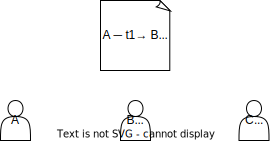
\includegraphics[]{img/blockchain/probleemstelling.pdf}
	\caption{\label{fig:probleemstelling}Probleemstelling}
\end{figure}

\begin{tcolorbox}[title=Voorbeeld]	
Partij A voert een transactie uit met partij B. Partij A schrijft de transactie weg in de ledger.

Partij C voert een transactie uit met partij A. Partij C schrijft de transactie weg in de ledger.
\end{tcolorbox}

Er schuilt een inherente vertrouwenskwestie in het bijhouden van een gedeelde ledger: alle deelnemedende partijen moeten elkaar vertrouwen. Volgende kwestie lijkt op het double-spendingprobleem bij cryptomunten:

\textbf{Probleem:} 
Partij A voert geen transactie uit met partij B, maar schrijft toch een lijn weg in de ledger. Partij B is hier uiteraard niet mee akkoord. Voor partij C lijkt het alsof er nog een transactie plaatsvond tussen A en B.


\subsection{Centralized ledger}
\label{sub:centralized-ledger}

Voorgaande probleemstelling werd klassiek aangepakt vanuit een gecentraliseerd systeem. Er wordt een onafhankelijke partij ingeschakeld voor het bijhouden en bewaken van de ledger. Deze derde partij houdt de ledger bij op een centrale databank die raadpleegbaar is door alle andere partijen. Wie een transactie wilt wegschrijven in de ledger, doet een aanvraag die kan gecheckt worden. Op die manier waakt de centrale partij erover dat er enkel geldige en geverifieerde transacties in de ledger kunnen komen. 

Om te authenticiteit van een transactie aan te tonen wordt in de praktijk gebruik gemaakt van een \textit{digital signature}. Het vormt de oplossing voor het \textit{copy-pasteprobleem} dat werd aangehaald in subsectie \ref{sub:double-spending} - \nameref{sub:double-spending}. Door bij elke regel een unieke code te gegenereren op basis van een publieke en private sleutel, kan deze later geverifiëerd worden\footnote{Een diepgaandere uiteenzetting van \textit{digital signatures} is in dit onderzoek niet aan de orde.}. Net zoals een handtekening bij fysieke documenten, wordt zo de probleemstelling aangepakt.

\begin{figure}[H]
	\centering
	\includegraphics[]{img/blockchain/centralized-ledger.pdf}
	\caption{\label{fig:centralized-ledger}Centralized ledger}
\end{figure}

Merk op dat de probleemstelling in principe niet volledig opgelost is. De vertrouwenskwestie die partijen onderling hadden, is in zekere zin gewoon verschoven naar het nieuwe, centrale figuur. Dit kan gezien worden als een Single Point of Failure.

\textbf{Probleem:} 
Op vraag van partij A verwijdert het centrale figuur een voorgaande transactie tussen A en B. 
Aangezien dit de enige kopie is van de ledger is er gaan manier voor partij B om hierop terug te komen. Parij C weet niets over het hele scenario.

Met een gedistribueerd systeem kan men de nood aan een centrale authoriteit proberen vermijden.


\subsection{Distributed ledger}
\label{sub:distributed-ledger}

Om de nood aan een centrale opslagplaatst te omzeilen, zou elke partij een eigen kopie kunnen bijhouden van de gezamenlijke ledger. Zo kan elke partij over zijn kopie waken en valse transacties onderscheppen. Om een nieuwe regel toe te voegen aan de ledger, wordt een signaal \textbf{gebroadcast} op het netwerk. De ontvangende partijen hun versie van de ledger updaten. Hierdoor ontstaat echter een nieuw probleem.

\begin{figure}[H]
	\centering
	\includegraphics[]{img/blockchain/distributed-ledger.pdf}
	\caption{\label{fig:distributed-ledger}Distributed ledger}
\end{figure}

\textbf{Probleem:} Partij A voert een transactie uit met partij B, maar broadcast dit niet naar partij C. De ledger van partij C stemt niet meer overeen met die van A en B.

Hoewel het handig is dat elke partij zijn eigen versie van de gedeelde ledger heeft, laat dit een nieuwe vraag ontstaan: wat is ``de juiste'' versie? Om transacties correct bij te houden in een gedistribueerd systeem, is er nood aan een protocol, een technologie die deelnemende partijen een manier biedt om het eens te zijn over wat de correcte ledger is. Die technologie staat bekend als een blockchain.


\section{Basisprincipes van een blockchain}
\label{sec:sleutelprincipes-van-een-blokchain}

De blockchain kwam als oplossing voor het probleem dat beschreven wordt in sectie \ref{sub:distributed-ledger} - \nameref{sub:distributed-ledger}. Zoals reeds aangegeven, werd dit probleem voor het eerst opgelost bij de ontwikkeling van de Bitcoin. Om een gegrond inzicht te geven in de eigenschappen van een blockchain, is deze sectie opgedeeld in drie basisprincipes. De concrete invulling van die principes is gebaseerd op de oorspronkelijke implementatie door Nakamoto.

Volgende subsecties zullen aantonen hoe het vertrouwensprobleem bij een \textit{distributed ledger} kan opgelost worden door het gezamenlijk opstellen van een keten van datablokken: een proces genaamd mining.


\subsection{Blokken}
\label{sub:blokken}

Een eerste basisprincipe is dat de ledger wordt opgebouwd uit zogenaamde blokken die elk een apart deel van de transacties oplijsten. Deze blokken worden om de zoveel tijd gegenereerd door een proces dat ``mining'' genoemd wordt.

Tijdens het minen, wordt gedurende een beperkte tijdsspanne geluisterd naar de transacties die gebroadcast worden over het netwerk. Het blok houdt deze transacties dan bij onder de vorm van een Merkle Tree\footnote{Deze speciale binaire boom maakt handig gebruik van hashing om de transacties van het blok snel valideerbaar te maken. Deze datastructuur wordt uitsluitend gebruikt binnen een blok. Om verwarring te vermijden met de structuur van de blockchain als geheel, wordt deze verder niet besproken.}. Op die manier omvat het een uniek deel van de ledger. Wanneer de tijdslimiet verstreken is, kan de opbouw van het blok afgerond worden. Hierbij gebeuren nog een aantal essentiële stappen die in de volgende subsecties besproken worden. 

Wanneer een blok klaar is, wordt het in zijn geheel \textit{gebroadcast}, waarna het door de deelnemers van het netwerk kan geaccepteerd worden. Zo wordt de distributed ledger stuk per stuk aangevuld.
Om deze stukken aan elkaar te linken, zal elk blok ook een verwijzing krijgen naar zijn voorganger. Voor deze verwijzing wordt gebruik gemaakt van een cryptografische hashfunctie. 

\begin{figure}[H]
	\centering
	\includegraphics[]{img/blockchain/blokken.pdf}
	\caption{\label{fig:blokken}De gedeelde ledger, opgedeeld in zogenaamde blokken.}
\end{figure}

\subsection{Cryptohashes}
\label{sub:cryptografische-hashfunctie}

Naast een lijst van transacties, houdt elk blok ook een verwijzing bij naar het voorgaande blok. Deze verwijzing is onder de vorm van een hashwaarde die bepaald wordt door een hashfunctie zoals SHA256. Wanneer die functie een blok als input krijgt, geeft deze een binaire tekenreeks van vaste lengte als output. Die tekenreeks wordt dan gebruikt als verwijzing naar het voorgaande blok. Op die manier komt men tot een keten van blokken: een blockchain.

\begin{tikzpicture}[
	roundnode/.style={circle, draw=green!60, fill=green!5, very thick, minimum size=7mm},
	squarednode/.style={rectangle, draw=blue!60, fill=blue!5, very thick, minimum size=5mm},
	]
	%Nodes
	\node[squarednode,fill=none]  (blok1)        					    {Blok 1};
	\node[draw=none,fill=none]    (input)         [below=of blok1]       {110110110010...111};
	\node[draw=none,fill=none]    (output-length) [below=of input, yshift=25]		{\textit{n} bits};
	\node[squarednode]            (sha256) 		  [right=of input]       {SHA256()};
	\node[draw=none,fill=none]    (output)        [right=of sha256]		{011010100...111010101};
	\node[draw=none,fill=none]    (output-length) [below=of output, yshift=25]		{256 bits};
	
	% Calligraphic brace
	\draw [decorate, decoration = {calligraphic brace}] (input.south east) --  (input.south west);
	\draw [decorate, decoration = {calligraphic brace}] (output.south east) --  (output.south west);
	
	%Lines
	\draw[dotted] (blok1.south) -- (input.north);
	\draw[-stealth] (input.east) -- (sha256.west);
	\draw[-stealth] (sha256.east) -- (output.west);
	
\end{tikzpicture}

Voor elke input van de hashfunctie, kan eenvoudig de output bepaald worden. Toch is het geheel onwezenlijk om de inverse berekening te maken. Daarom wordt deze hashfunctie cryptografisch genoemd. Dit is een van de sleutelkenmerken die blockchain mogelijk maken: het is niet haalbaar om de input van een gegeven hashwaarde te \textit{reverse-engineeren}. 

Het is belangrijk om erop te wijzen dat zelfs de kleinste wijziging aan de input van een hashfunctie, een drastisch verschil maakt aan de output. In deze context betekent dit dat een wijziging aan een blok (hoe klein dan ook) ervoor zorgt dat zijn hashwaarde volledig verandert. Aangezien deze hashwaarden gebruikt worden om de blokken aan elkaar te ketenen, zal de blockchain hierdoor ergens doorbroken worden. De hashwaarde die naar dit blok verwees is namelijk niet meer correct. Om terug tot een geldige blockchain te komen zal er een hele kettingreactie moeten plaatsvinden. Onderstaand voorbeeld illustreert waarom dit het geval is:

\begin{tcolorbox}[title=Voorbeeld]	
	\begin{tikzpicture}[every node/.style={inner sep=0,outer sep=0, font=\small}, align=left, node distance=.5]
		
		%Nodes
		\node[draw=none,fill=none] (11)        					    {\textbf{Stel: }};
		\node[draw=none,fill=none] (12) [right=of 11, xshift=-15] {Er wordt een wijziging aangebracht aan Blok 1.};
		\node[draw=none,fill=none] (13) [below=of 12.west, anchor=west, xshift=23] {De cryptohash van Blok 1 verandert.};
		\node[draw=none,fill=none] (21) [below=of 13.west, anchor=west, xshift=-46, yshift=-10]  {De prev\_block-verwijzing van Blok2 naar Blok1 moet geüpdatet worden.};
		\node[draw=none,fill=none] (22) [below=of 21.west, anchor=west, xshift=23]  {M.a.w.: er wordt een wijziging aangebracht aan Blok 2.};
		\node[draw=none,fill=none] (23) [below=of 22.west, anchor=west, xshift=23]  {De cyptohash van Blok 2 verandert.};
		\node[draw=none,fill=none] (31) [below=of 23.west, anchor=west, xshift=-46, yshift=-10]  {De prev\_block-verwijzing van Blok3 naar Blok2 moet geüpdatet worden.};
		\node[draw=none,fill=none] (32) [below=of 31.west, anchor=west, xshift=23]  {M.a.w.: er wordt een wijziging aangebracht aan Blok 3.};
		\node[draw=none,fill=none] (33) [below=of 32.west, anchor=west, xshift=23]  {De cyptohash van Blok 3 wordt opnieuw berekend};
		\node[draw=none,fill=none] (41) [below=of 33.west, anchor=west, xshift=-46, yshift=-10]  {...};
		
		%Lines
		\draw[->] (12.south west) .. controls +(down:3mm) and +(left:3mm) .. (13.west);
		\draw[->] (13.south west) .. controls +(left:3mm) and +(up:6mm) .. (21.north west);
		\draw[->] (21.south west) .. controls +(down:3mm) and +(left:3mm) .. (22.west);
		\draw[->] (22.south west) .. controls +(down:3mm) and +(left:3mm) .. (23.west);
		\draw[->] (23.south west) .. controls +(left:3mm) and +(up:6mm) .. (31.north west);
		\draw[->] (31.south west) .. controls +(down:3mm) and +(left:3mm) .. (32.west);
		\draw[->] (32.south west) .. controls +(down:3mm) and +(left:3mm) .. (33.west);
		\draw[->] (33.south west) .. controls +(left:3mm) and +(up:6mm) .. (41.north west);
	\end{tikzpicture}	
\end{tcolorbox}

Bovenstaand voorbeeld toont aan dat de inhoud van een blok niet gewijzigd kan worden, zonder ook alle daaropvolgende blokken te wijzigen. Het gaat namelijk steeds gepaard met de wijziging van de bijhorende hash. Aangezien deze hash altijd deel uitmaakt van een daaropvolgend blok, zullen al deze verwijzingen moeten herberekend worden.

Niemand zal nog een aanpassing kunnen maken aan de ledger zoals:
\begin{itemize}
	\item een transactie wijzigen, toegevoegen of verwijderen;
	\item het verwisselen van transacties;
	\item het verwisselen van blokken;
\end{itemize}

Zonder verantwoordelijk te worden voor alle hashverwijzingen na het geïmpacteerde punt. Op die manier wordt al een eerste stap gezet naar een onvervalsbare, of \textit{immutable} \textit{distributed ledger}. Het doel is echter nog niet bereikt.

\textbf{Probleem:} Wie de ledger wenst te vervalsen hoeft zich geen zorgen te maken over het doorbreken van de keten. 
Door simpelweg de nodige hashes opnieuw te berekenen, komt men uiteindelijk terug tot een geldige blockchain. Dat kan, aangezien een hashfunctie mermaal uitvoeren geen zware taak is. Op die manier kunnen nog steeds tegenstrijdige, maar technisch geldige ledgers ontstaan.

Een laatste essentieel principe bestaat eruit om bij elk blok een extra speciaal stuk data te eisen, waardoor het vinden van een gepaste hash wel een rekenintesieve opdracht wordt. Op die manier wordt ook het bovenstaande probleem opgelost.

\begin{figure}[H]
	\centering
	\includegraphics[]{img/blockchain/blokken-met-cryptohash.pdf}
	\caption{\label{fig:blokken-met-cryptohash}Blokken die naar elkaar verwijzen met behulp van een cryptohash.}
\end{figure}

\subsection{Proof of Work}
\label{sub:proof-of-work}

De laatste sleutel bestaat eruit om een extra stukje data toe te voegen aan elk blok genaamd de ``Proof of Work''.
Afhankelijk van de inhoud van die Proof of Work, zal het blok uiteraard veranderen, en als gevolg ook de hash van dat blok. Met andere woorden: door met dit stukje data te ``spelen'', wijzigt men de hash die nodig is om te verwijzen naar dat blok.

Het opzet is om nu een extra vereiste op te leggen aan die hashverwijzingen, zodat het tijdrovend wordt om die PoW te produceren. Nakamoto vond een dergelijke vereiste, die desondanks eenvoudig is om te verifiëren: de has moet beginnen met een voorgedefiniëerd aantal nul-bits. Een blok zal pas als geldig beschouwd worden, wanneer de eerste \textit{n} bits allemaal de waarde nul hebben. 

\begin{tikzpicture}[
	roundnode/.style={circle, draw=green!60, fill=green!5, very thick, minimum size=7mm},
	squarednode/.style={rectangle, draw=blue!60, fill=blue!5, very thick, minimum size=5mm},
	]
	%Nodes
	\node[squarednode,fill=none, align=center]  (blok1)        					    {Blok 1\\\textbf{incl. POW}};
	\node[draw=none,fill=none]    (input)         [below=of blok1]       {011001111010...111};
	\node[draw=none,fill=none]    (output-length) [below=of input, yshift=25]		{\textit{n} bits};
	\node[squarednode]            (sha256) 		  [right=of input]       {SHA256()};
	\node[draw=none,fill=none]    (output)        [right=of sha256]		{\textbf{000000000}...111010101};
	\node[draw=none,fill=none]    (output-length) [below=of output, yshift=25]		{256 bits};
	
	% Calligraphic brace
	\draw [decorate, decoration = {calligraphic brace}] (input.south east) --  (input.south west);
	\draw [decorate, decoration = {calligraphic brace}] (output.south east) --  (output.south west);
	
	%Lines
	\draw[dotted] (blok1.south) -- (input.north);
	\draw[-stealth] (input.east) -- (sha256.west);
	\draw[-stealth] (sha256.east) -- (output.west);
\end{tikzpicture}

Om tot een geldig blok te komen, zal dus telkens een PoW-waarde gezocht moeten worden, die de hash van dat blok laat starten met de nodige nulbits. Aangezien het hier over een cryptografische hasahfunctie gaat, valt die PoW niet zomaar te voorspellen. Er zit niets anders op dan herhaaldelijk willekeurige waarden uit te proberen, tot er toevallig een geldige hashwaarde uit voortkomt.

``The proof-of-work involves scanning for a value that when hashed, such as with SHA-256, the hash begins with a number of zero bits. The average work required is exponential in the number of zero bits required and can be verified by executing a single hash.'' (Nakamoto)

Onderstaand voorbeeld illustreert hoe de kettingreactie bij het wijzigen van een blok er nu uitziet:

\begin{tcolorbox}[title=Voorbeeld]	
	\begin{tikzpicture}[every node/.style={inner sep=0,outer sep=0, font=\small}, align=left, node distance=.5]
		
		%Nodes
		\node[draw=none,fill=none] (11)        					    {\textbf{Stel: }};
		\node[draw=none,fill=none] (12) [right=of 11, xshift=-15] {Er wordt een wijziging aangebracht aan Blok 1.};
		\node[draw=none,fill=none] (13) [below=of 12.west, anchor=west, xshift=23] {De cryptohash van Blok 1 verandert naar een ongeldige waarde.};
		\node[draw=none,fill=none] (14) [below=of 13.west, anchor=west, xshift=23] {Er moet opnieuw een PoW gezocht worden voor Blok1.};
		\node[draw=none,fill=none] (15) [below=of 14.west, anchor=west, xshift=23] {De cryptohash van Blok1 verandert naar een geldige waarde.};
		\node[draw=none,fill=none] (21) [below=of 15.west, anchor=west, xshift=-92, yshift=-10]  {De prev\_block-verwijzing van Blok2 naar Blok1 moet geüpdatet worden.};
		\node[draw=none,fill=none] (22) [below=of 21.west, anchor=west, xshift=23]  {M.a.w.: er wordt een wijziging aangebracht aan Blok 2.};
		\node[draw=none,fill=none] (23) [below=of 22.west, anchor=west, xshift=23]  {De cyptohash van Blok 2 verandert naar een ongeldige waarde.};
		\node[draw=none,fill=none] (24) [below=of 23.west, anchor=west, xshift=23] {Er moet opnieuw een PoW gezocht worden voor Blok2.};
		\node[draw=none,fill=none] (25) [below=of 24.west, anchor=west, xshift=23] {De cryptohash van Blok2 verandert naar een geldige waarde.};
		\node[draw=none,fill=none] (31) [below=of 25.west, anchor=west, xshift=-92, yshift=-10]  {De prev\_block-verwijzing van Blok3 naar Blok2 moet geüpdatet worden.};
		\node[draw=none,fill=none] (32) [below=of 31.west, anchor=west, xshift=23]  {M.a.w.: er wordt een wijziging aangebracht aan Blok 3.};
		\node[draw=none,fill=none] (33) [below=of 32.west, anchor=west, xshift=23]  {De cyptohash van Blok 3 verandert  naar een ongeldige waarde.};
		\node[draw=none,fill=none] (34) [below=of 33.west, anchor=west, xshift=23] {Er moet opnieuw een PoW gezocht worden voor Blok3.};
		\node[draw=none,fill=none] (35) [below=of 34.west, anchor=west, xshift=23] {De cryptohash van Blok3 verandert naar een geldige waarde.};
		\node[draw=none,fill=none] (41) [below=of 35.west, anchor=west, xshift=-92, yshift=-10]  {...};
		
		%Lines
		\draw[->] (12.south west) .. controls +(down:3mm) and +(left:3mm) .. (13.west);
		\draw[->] (13.south west) .. controls +(down:3mm) and +(left:3mm) .. (14.west);
		\draw[->] (14.south west) .. controls +(down:3mm) and +(left:3mm) .. (15.west);
		\draw[->] (15.south west) .. controls +(left:3mm) and +(up:6mm) .. (21.north west);
		\draw[->] (21.south west) .. controls +(down:3mm) and +(left:3mm) .. (22.west);
		\draw[->] (22.south west) .. controls +(down:3mm) and +(left:3mm) .. (23.west);
		\draw[->] (23.south west) .. controls +(down:3mm) and +(left:3mm) .. (24.west);
		\draw[->] (24.south west) .. controls +(down:3mm) and +(left:3mm) .. (25.west);
		\draw[->] (25.south west) .. controls +(left:3mm) and +(up:6mm) .. (31.north west);
		\draw[->] (31.south west) .. controls +(down:3mm) and +(left:3mm) .. (32.west);
		\draw[->] (32.south west) .. controls +(down:3mm) and +(left:3mm) .. (33.west);
		\draw[->] (33.south west) .. controls +(down:3mm) and +(left:3mm) .. (34.west);
		\draw[->] (34.south west) .. controls +(down:3mm) and +(left:3mm) .. (35.west);
		\draw[->] (35.south west) .. controls +(left:3mm) and +(up:6mm) .. (41.north west);
	\end{tikzpicture}	
\end{tcolorbox}


Een wijziging aan een blok zorgt er dus nog steeds voor dat alle daaropvolgende hashes herevalueerd moeten worden. Door de toevoeging van de PoW is die herevaluatie nu ook een rekenintesieve opdracht geworden. Om een verwijzing te herstellen moet namelijk steeds opnieuw een geldige hashwaarde gevonden worden. Om die te vinden moet gescand worden naar een gepaste PoW-waarde.

\begin{figure}[H]
	\centering
	\includegraphics[]{img/blockchain/blokken-met-pow.pdf}
	\caption{\label{fig:blokken-met-pow}Proof of Work als onderdeel van de blokken.}
\end{figure}


